\documentclass{standalone}
\usepackage{tikz}
\usetikzlibrary{patterns, positioning}
\usepackage[sfdefault]{ClearSans} %% option 'sfdefault' activates Clear Sans as the default text font
\usepackage[T1]{fontenc}

\begin{document}
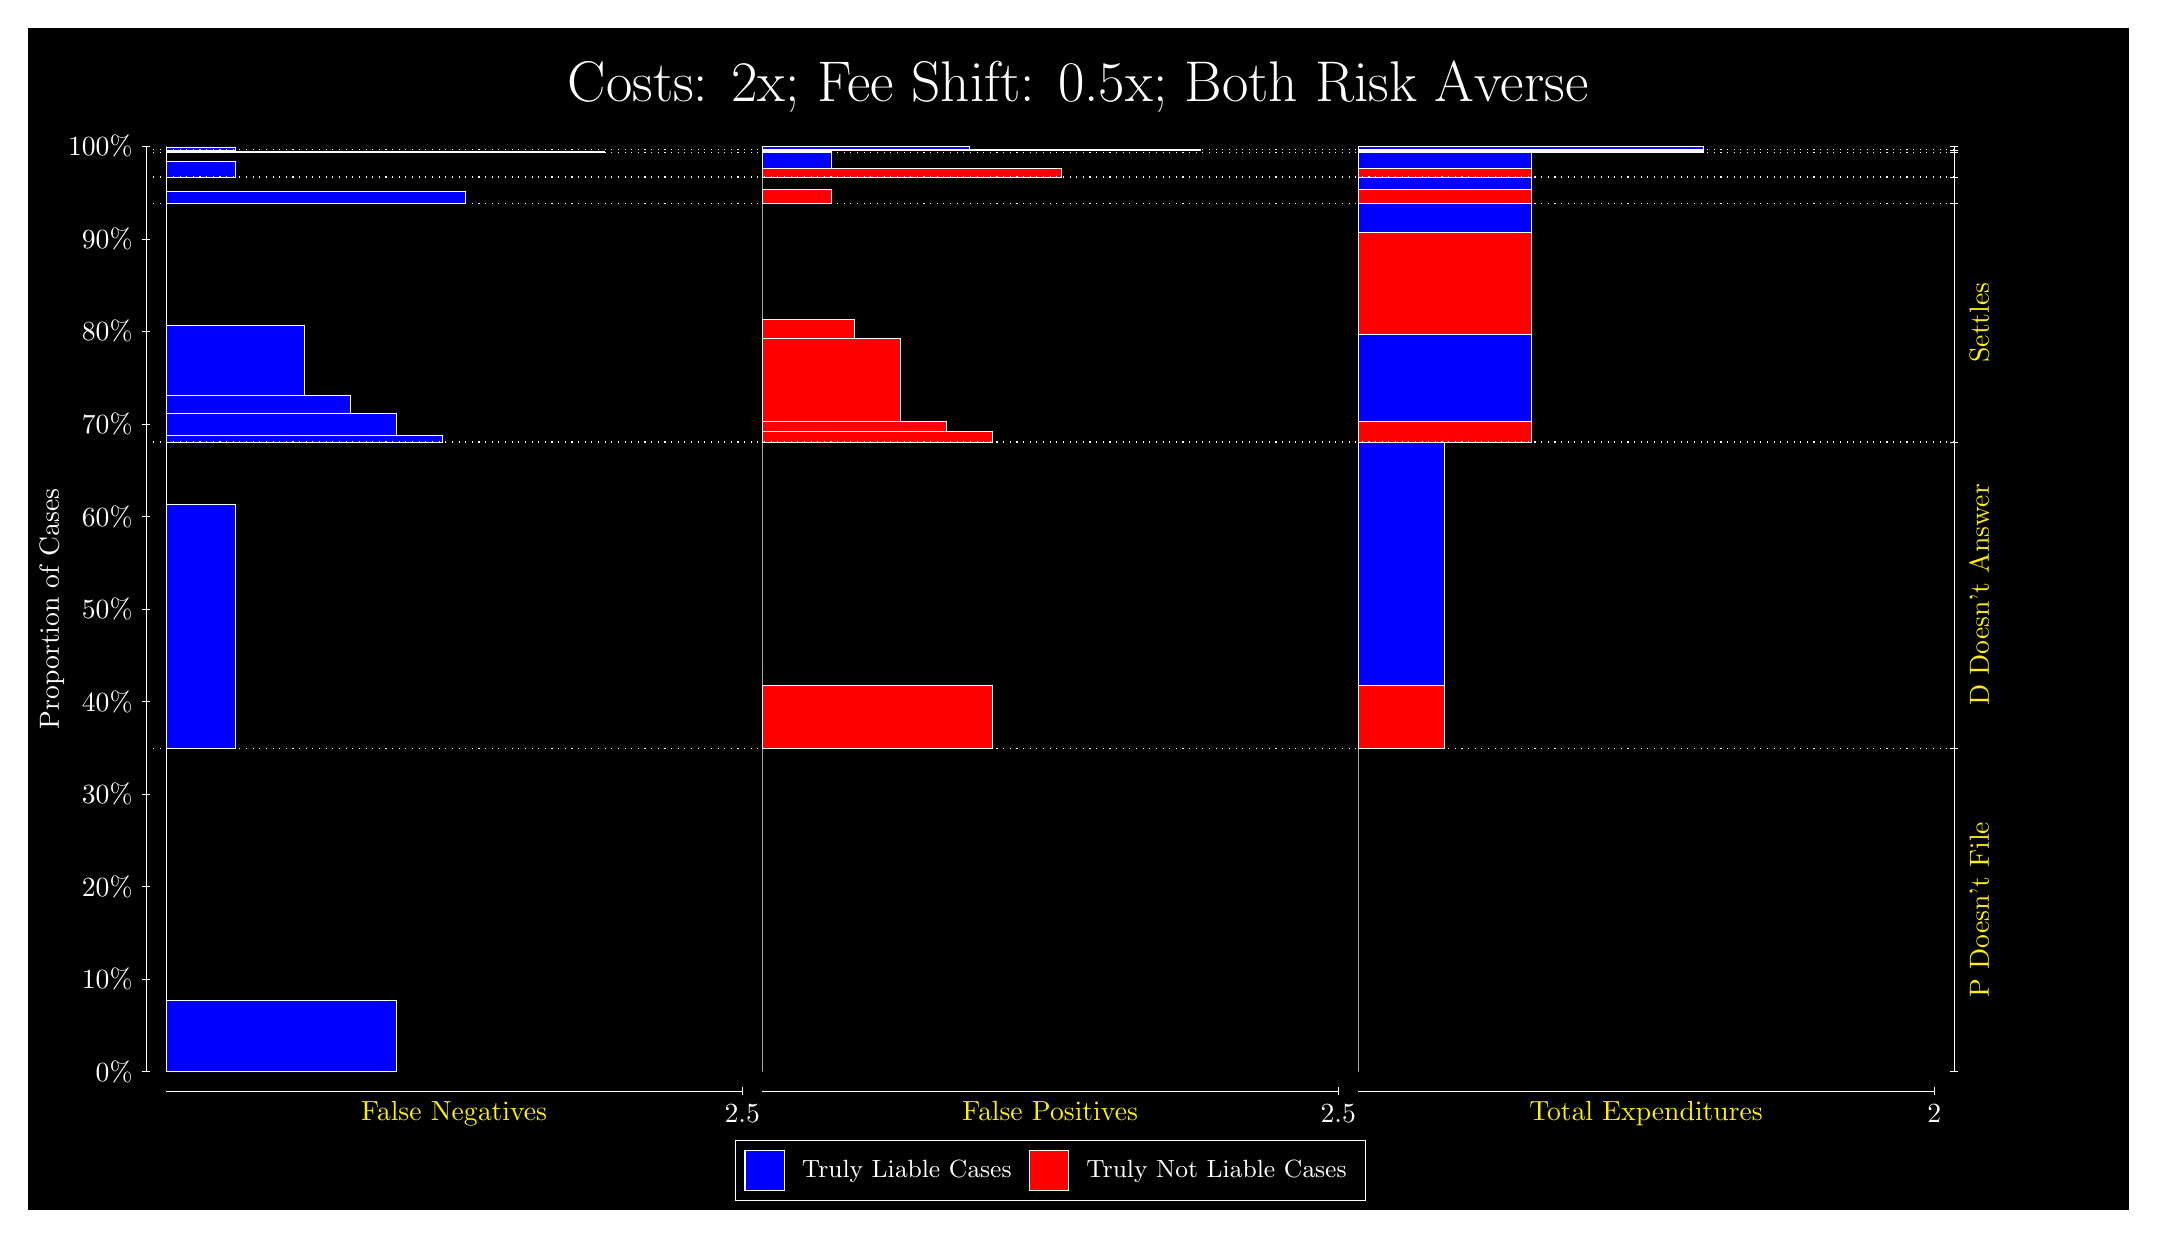
\begin{tikzpicture}
\draw[fill=black] (0,0) rectangle (26.667,15);
\draw[text=white] (0,13.5) rectangle (26.667,15) node[midway] {\huge Costs: 2x; Fee Shift: 0.5x; Both Risk Averse};
\draw[white, very thin] (1.5,1.75) -- (1.5,13.5);
\node[rotate=90, text=white, anchor=center] at (0.3, 7.625) {Proportion of Cases};
\draw[white, very thin] (1.45,1.75) -- (1.55,1.75);
\node[text=white, anchor=east] at (1.45, 1.75) {0\%};
\draw[white, very thin] (1.45,2.925) -- (1.55,2.925);
\node[text=white, anchor=east] at (1.45, 2.925) {10\%};
\draw[white, very thin] (1.45,4.1) -- (1.55,4.1);
\node[text=white, anchor=east] at (1.45, 4.1) {20\%};
\draw[white, very thin] (1.45,5.275) -- (1.55,5.275);
\node[text=white, anchor=east] at (1.45, 5.275) {30\%};
\draw[white, very thin] (1.45,6.45) -- (1.55,6.45);
\node[text=white, anchor=east] at (1.45, 6.45) {40\%};
\draw[white, very thin] (1.45,7.625) -- (1.55,7.625);
\node[text=white, anchor=east] at (1.45, 7.625) {50\%};
\draw[white, very thin] (1.45,8.8) -- (1.55,8.8);
\node[text=white, anchor=east] at (1.45, 8.8) {60\%};
\draw[white, very thin] (1.45,9.975) -- (1.55,9.975);
\node[text=white, anchor=east] at (1.45, 9.975) {70\%};
\draw[white, very thin] (1.45,11.15) -- (1.55,11.15);
\node[text=white, anchor=east] at (1.45, 11.15) {80\%};
\draw[white, very thin] (1.45,12.325) -- (1.55,12.325);
\node[text=white, anchor=east] at (1.45, 12.325) {90\%};
\draw[white, very thin] (1.45,13.5) -- (1.55,13.5);
\node[text=white, anchor=east] at (1.45, 13.5) {100\%};

\draw[white, very thin] (24.457,1.75) -- (24.457,13.5);
\draw[white, very thin] (24.407,1.75) -- (24.507,1.75);
\node[anchor=west] at (24.407, 1.75) {};
\draw[white, very thin] (24.407,5.858) -- (24.507,5.858);
\node[anchor=west] at (24.407, 5.858) {};
\draw[white, very thin] (24.407,9.7454) -- (24.507,9.7454);
\node[anchor=west] at (24.407, 9.7454) {};
\draw[white, very thin] (24.407,12.778) -- (24.507,12.778);
\node[anchor=west] at (24.407, 12.778) {};
\draw[white, very thin] (24.407,13.11) -- (24.507,13.11);
\node[anchor=west] at (24.407, 13.11) {};
\draw[white, very thin] (24.407,13.423) -- (24.507,13.423);
\node[anchor=west] at (24.407, 13.423) {};
\draw[white, very thin] (24.407,13.455) -- (24.507,13.455);
\node[anchor=west] at (24.407, 13.455) {};
\draw[white, very thin] (24.407,13.5) -- (24.507,13.5);
\node[anchor=west] at (24.407, 13.5) {};

\draw[white, very thin, fill=blue] (1.75,1.75) rectangle (4.6775,2.6527);
\draw[white, very thin, fill=red] (1.75,2.6527) rectangle (1.75,5.858);
\draw[white, very thin, fill=blue] (1.75,5.858) rectangle (2.6283,8.953);
\draw[white, very thin, fill=red] (1.75,8.953) rectangle (1.75,9.7454);
\draw[white, very thin, fill=blue] (1.75,9.7454) rectangle (5.2631,9.8273);
\draw[white, very thin, fill=blue] (1.75,9.8273) rectangle (4.6775,10.115);
\draw[white, very thin, fill=blue] (1.75,10.115) rectangle (4.092,10.341);
\draw[white, very thin, fill=blue] (1.75,10.341) rectangle (3.5065,11.221);
\draw[white, very thin, fill=red] (1.75,11.221) rectangle (1.75,12.778);
\draw[white, very thin, fill=blue] (1.75,12.778) rectangle (5.5558,12.93);
\draw[white, very thin, fill=red] (1.75,12.93) rectangle (1.75,13.11);
\draw[white, very thin, fill=blue] (1.75,13.11) rectangle (2.6283,13.315);
\draw[white, very thin, fill=red] (1.75,13.315) rectangle (1.75,13.423);
\draw[white, very thin, fill=blue] (1.75,13.423) rectangle (7.3123,13.435);
\draw[white, very thin, fill=red] (1.75,13.435) rectangle (1.75,13.455);
\draw[white, very thin, fill=blue] (1.75,13.455) rectangle (2.6283,13.488);
\draw[white, very thin, fill=red] (1.75,13.488) rectangle (1.75,13.5);
\draw[white, very thin, fill=red] (9.3189,1.75) rectangle (9.3189,4.9553);
\draw[white, very thin, fill=blue] (9.3189,4.9553) rectangle (9.3189,5.858);
\draw[white, very thin, fill=red] (9.3189,5.858) rectangle (12.246,6.6505);
\draw[white, very thin, fill=blue] (9.3189,6.6505) rectangle (9.3189,9.7454);
\draw[white, very thin, fill=red] (9.3189,9.7454) rectangle (12.246,9.8798);
\draw[white, very thin, fill=red] (9.3189,9.8798) rectangle (11.661,10.006);
\draw[white, very thin, fill=red] (9.3189,10.006) rectangle (11.075,11.059);
\draw[white, very thin, fill=red] (9.3189,11.059) rectangle (10.49,11.303);
\draw[white, very thin, fill=blue] (9.3189,11.303) rectangle (9.3189,12.778);
\draw[white, very thin, fill=red] (9.3189,12.778) rectangle (10.197,12.958);
\draw[white, very thin, fill=blue] (9.3189,12.958) rectangle (9.3189,13.11);
\draw[white, very thin, fill=red] (9.3189,13.11) rectangle (13.125,13.218);
\draw[white, very thin, fill=blue] (9.3189,13.218) rectangle (10.197,13.423);
\draw[white, very thin, fill=red] (9.3189,13.423) rectangle (10.197,13.443);
\draw[white, very thin, fill=blue] (9.3189,13.443) rectangle (9.3189,13.455);
\draw[white, very thin, fill=red] (9.3189,13.455) rectangle (14.881,13.467);
\draw[white, very thin, fill=blue] (9.3189,13.467) rectangle (11.954,13.5);
\draw[white, very thin, fill=red] (16.888,1.75) rectangle (16.888,4.9553);
\draw[white, very thin, fill=blue] (16.888,4.9553) rectangle (16.888,5.858);
\draw[white, very thin, fill=red] (16.888,5.858) rectangle (17.986,6.6505);
\draw[white, very thin, fill=blue] (16.888,6.6505) rectangle (17.986,9.7454);
\draw[white, very thin, fill=red] (16.888,9.7454) rectangle (19.083,10.006);
\draw[white, very thin, fill=blue] (16.888,10.006) rectangle (19.083,11.112);
\draw[white, very thin, fill=red] (16.888,11.112) rectangle (19.083,12.408);
\draw[white, very thin, fill=blue] (16.888,12.408) rectangle (19.083,12.778);
\draw[white, very thin, fill=red] (16.888,12.778) rectangle (19.083,12.958);
\draw[white, very thin, fill=blue] (16.888,12.958) rectangle (19.083,13.11);
\draw[white, very thin, fill=red] (16.888,13.11) rectangle (19.083,13.218);
\draw[white, very thin, fill=blue] (16.888,13.218) rectangle (19.083,13.423);
\draw[white, very thin, fill=red] (16.888,13.423) rectangle (21.279,13.443);
\draw[white, very thin, fill=blue] (16.888,13.443) rectangle (21.279,13.455);
\draw[white, very thin, fill=red] (16.888,13.455) rectangle (21.279,13.467);
\draw[white, very thin, fill=blue] (16.888,13.467) rectangle (21.279,13.5);
\draw[white, dotted] (1.5,5.858) -- (24.457,5.858);
\draw[white, dotted] (1.5,9.7454) -- (24.457,9.7454);
\draw[white, dotted] (1.5,12.778) -- (24.457,12.778);
\draw[white, dotted] (1.5,13.11) -- (24.457,13.11);
\draw[white, dotted] (1.5,13.423) -- (24.457,13.423);
\draw[white, dotted] (1.5,13.455) -- (24.457,13.455);
\draw[white, very thin] (1.75,1.5) -- (9.0689,1.5);
\node[text=yellow, anchor=north] at (5.4094, 1.5) {False Negatives};
\draw[white, very thin] (9.0689,1.45) -- (9.0689,1.55);
\node[text=white, anchor=north] at (9.0689, 1.45) {2.5};

\draw[white, very thin] (9.3189,1.5) -- (16.638,1.5);
\node[text=yellow, anchor=north] at (12.978, 1.5) {False Positives};
\draw[white, very thin] (16.638,1.45) -- (16.638,1.55);
\node[text=white, anchor=north] at (16.638, 1.45) {2.5};

\draw[white, very thin] (16.888,1.5) -- (24.207,1.5);
\node[text=yellow, anchor=north] at (20.547, 1.5) {Total Expenditures};
\draw[white, very thin] (24.207,1.45) -- (24.207,1.55);
\node[text=white, anchor=north] at (24.207, 1.45) {2};

\node[text=yellow, centered, rotate=90] at (24.777, 3.804) {P Doesn't File};
\node[text=yellow, centered, rotate=90] at (24.777, 7.8017) {D Doesn't Answer};
\node[text=yellow, centered, rotate=90] at (24.777, 11.262) {Settles};





\draw (12.978300999999998,1.5) node[draw=none] (baseCoordinate) {};
\begin{scope}[align=center]
        \matrix[scale=0.5, draw=white, below=0.5cm of baseCoordinate, nodes={draw}, column sep=0.1cm]{
            \node[rectangle, draw, minimum width=0.5cm, minimum height=0.5cm, fill=blue] {}; &
            \node[draw=none, font=\small, text=white] (B) {Truly Liable Cases}; &
            \node[rectangle, draw, minimum width=0.5cm, minimum height=0.5cm, fill=red] {}; &
            \node[draw=none, font=\small, text=white] (B) {Truly Not Liable Cases}; \\
            };
\end{scope}

\end{tikzpicture}
\end{document}